\chapter{Огляд методів та задач електродинаміки у часовій області}
\label{ch:review}

%%%%%%%%%%%%%%%%%%%%%%%%%%%%%%%%%%%%%%%%%%%%%%%%%%%%%%%%%%%%%%%%%%%%%%%%%%%%%%
\section{Сучасна імпульсна та надширокосмугова радіофізика}

% Розвиток науки і техніки
% Наслідком історичної ґенези радіотехнічного обладнання
Підхід частотної селекції інформації набув масового поширення в радіофізиці
перебігом історії XX-го століття \cite{imp:Nosich2001}. Проте, вимоги 
сучасності до радіотехнічних приладів значно підвищились: з'явилась потреба 
у створенні нових засобів комунікації та локації. Зокрема, одним із 
способів покращення технічних характеристик радіоапаратури стало 
використання надширокосмугових режимів роботи, а на початку XXI-го 
століття було закладено практичне застосування нелінійної природи 
надширокосмугових електромагнітних процесів \cite{imp:Chernogor2008}.

Імпульсні та надширокосмугові коливання, що мають електромагнітну природу, 
вивчаються таким розділом фізики як нестаціонарна електродинаміка. Прийнято 
розділяти поняття імпульсного та надширокосмугового поля -- імпульсне поле 
не завжди називають надширокосмуговим. Згідно з рішенням федеральної 
комісії зв'язку США від 2007 року \cite{imp:RadarStandard2007}, 
надширокосмуговим називається коливання електромагнітної енергії, 
відносна ширина спектра якого принаймні вища за $ 25\% $, тобто:

\begin{equation} \label{eq:spectum_width}
\eta = \frac{f_{max} - f_{min}}{f_{max} + f_{min}} > 0.25,
\end{equation}
%
де $ f_{max} $ -- максимальна частота спектру сигналу, а $ f_{min} $ -- 
мінімальна частота спектру. Надалі користуватимемось цим визначенням. 
Хоча границі спектру реального сигналу досить умовні, існують декілька 
загальновизнаних способів їх визначити, серед яких найчастіше 
використовується рівень половинної енергії спектру ($ 0.707 $ за 
амплітудно-частотною характеристикою).

В природі спостерігати надширокосмугові електромагнітні хвилі можливо при 
ядерних реакціях \cite{imp:Baum2007}, при проходженні сонячного термінатора, 
при атмосферних явищах \cite{imp:Uman2006}, землетрусах 
\cite{imp:Hayakawa2008} тощо. Крім того, фоновий електромагнітний шум і 
власні завади радіотехнічного обладнання найчастіше мають 
надширокосмугову природу. Широка розповсюдженість таких явищ в 
навколишньому середовищі слугує аргументом на користь ефективності 
застосування надширокосмугових хвиль в науці і техніці.

Імпульсні радіохвилі штучно формують двома підходами: випромінюють антеною 
з низькою добротністю обмежений в часі гармонійний сигнал 
\cite{imp:Mesyas1963, imp:Mesyas1974} або стрибковий розряд електричного 
струму \cite{imp:BaumMN053}. Антено-фідерна система, для задовольняння 
умови низької добротності, виготовляється з максимально схожими 
характеристиками на широкому спектрі частот. Якщо спектр сформованого в 
такий спосіб електромагнітного коливання не задовольняє умові 
мінімальної ширини спектру \eqref{eq:spectum_width}, то його називають 
радіоімпульсом, який не розгладяться в даній роботі.

На практиці, однією з найважливіших якісних характеристик надширокосмугових
радіотехнічних пристроїв виявилась тривалість імпульсу. Імпульси меншої 
тривалості дозволяють, насамперед, концентрувати більшу кількість енергії,
що важливо, наприклад, для галузі медичної діагностики 
\cite{imp:Guardiola2010}. Також, менша тривалість імпульсу надає 
можливість передавати більшу кількість цифрових даних через радіоканал, що 
напряму витікає з формули Хартлі \cite{imp:Taub1986}. За тривалість 
випроміненого імпульсу відповідає цілий ряд параметрів серед яких і 
параметри антени, але визначальний вплив має електронний ключ, що подає 
струм живлення на антено-фідерну систему замикаючи, а інколи і розмикаючи 
електричне коло.

% нові фізичні принципи

Основним фактором, що підбурює інтерес до надширокосмугових систем є 
теоретична можливість поєднати особливості електромагнітного випромінювання 
на різних частотних діапазонах, що дозволить покращити характеристики 
існуючих радіоелектронних систем та розширить сферу їх застосування.
Наприклад, у 2019 році імпульсну надширокосмугову однокристальну 
радіосистему було вперше вбудовано у пристрій стільникового зв'язку 
Apple iPhone 11 Pro. Також, використання надширокосмугових імпульсних 
хвиль, дозволяє розв'язати неможливі для вузькодіапазонних приладів 
технічні задачі. Деякі з таких технічних задач вже загальнодоступні на
ринку споживацької електроніки, наприклад:

\begin{enumerate}

\item автомобільний радар малої дальності дії - допоміжний засіб 
технічного зору для автопілотів п'ятого покоління, що здатен працювати 
з потрібною точністю у несприятливих погодних умовах, а тобто в 
дисперсному, поглинальному і провідному середовищі \cite{imp:Yarovoy2017};

\item пристрій підводного радіозв'язку - засіб бездротової 
телекомунікації для систем зв'язку, де один або більше учасників 
зв'язку, занурені у провідне середовище \cite{imp:Garcia2009, 
imp:Karagianni2015}.

% \item Засіб вимірювання товщини та якості фарби (толщік)
% \item Кліматичний радар
\end{enumerate}

Завдяки відсутності носійної хвилі і роботі передавача в імпульсному режимі 
значно скорочується споживання електричної енергії передавачем, що породило 
значний інтерес до використання фізичних принципів випромінювання 
надширокосмугових сигналів в галузі техніки інтернету речей (IoT). 
Сучасні мережеві протоколи канального рівня стеку TCP/IP, такі як WiFi6 
(IEEE 802.11ax) \cite{imp:Khorov2019} використовують саме радіоімпульси,
як носій інформації, що негативно впливає на споживання електричної енергії.

Також, з початку 60-х років технічні засоби, робота яких базується на 
використанні надширокосмугових електромагнітних хвиль, активно 
використовуються військовими. Серед таких досліджень варто відмітити 
науково-дослідницький проект ATLAS-1 під керівництвом К. Баума 
\cite{imp:BaumSSN0267}, який було спрямовано на захист устаткування 
літальних апаратів від електромагнітного уражаючого фактору ядерного 
вибуху.

Окремим напрямком використання надширокосмугових радіолокаційних систем 
стало їх застосування для систем внутрішнього позиціювання (IPS), що у 
поєднанні з методикою технічного зору SLAM (одночасна локалізація і 
картографування) дозволяє отримувати тривимірну мапу внутрішнього 
середовища \cite{imp:Segura2011}. Аналогічна система внутрішнього 
позиціювання, що базується використанні гармонійних сигналів 
характеризується меншою точністю \cite{imp:Zou2017}.

%%%%%%%%%%%%%%%%%%%%%%%%%%%%%%%%%%%%%%%%%%%%%%%%%%%%%%%%%%%%%%%%%%%%%%%%%%%%%%
\section{Застосування теорії збурень для лінеаризації нелінійних задач}

В фізичній науці прийнято розглядати замкнені енергетичні системи як для 
дослідження природних явищ так і задля розв'язання практичних задач. 
Отримати постанову замкненої задачі дозволяє нехтування деякими взаємодіями. 
Так, при розв'язані задачі поширення електромагнітних хвиль в середовищі, 
майже завжди спрощують вплив електромагнітної енергії на молекулярні та
всерединоатомні явища до лінійного закону індукції. Так, при малих потенціалах 
та повільних змінах потенціалу отримані модельні дані підтверджуються 
емпірично, але починаючи від деяких амплітудних та спектральних характеристик 
поля спостерігаються значні розбіжності між модельними та емпіричними 
даними. Для сучасної фізики очевидно, що такі прояви пов'язання зі 
зростанням внеску деяких ефектів зі зростанням енергії процесу. Нелінійна 
фізика займається дослідженням природи та описом таких явищ. Звісно, 
розглядаючи систему на макрорівні, також можна досягти досить точного 
моделювання, але в цьому випадку складність розв'язання задачі також 
зростає. На щастя апарат нелінійної фізики дозволяє значно спростити 
фізичну модель сильного процесу, а тобто процесу енергія якого достатня 
для збурення неврахованих макромоделлю мікроявищ. Нелінійність взаємодії
імпульсних електромагнітних хвиль з середовищем явище досить 
поширене через те, що імпульсне поле локалізує в  часі велику кількість 
енергії.

Солітон -- нестаціонарне нелінійне явище, поширене в сучасних 
задачах електродинаміки та цікаве для наукової спільноти. Перша згадка 
поняття солітон пов'язується з дослідженням поширення нелінійної поверхневої 
механічної хвилі з характерною довжиною хвилі, яка значно перевищує глибину 
водойми. Отримане в цьому дослідженні Корвегом і де Візом рівняння, пізніше 
назване на честь дослідників, пов'язало нелінійність деякого параметру хвилі 
та дисперсійні властивості середовища, як необхідні умови появи солітону.
Таким чином взявши за основу аналітичне лінійне розв'язання задачі поширення 
нестаціонарної електромагнітної хвилі та врахувавши дисперсійні і нелінійні 
ефекти взаємодії з середовищем можна дослідити процес формування 
солітоноподібних явищ.

Аналітичним описом нелінійного процесу виступає нелінійне диференціальне чи 
інтегро-диференціальне рівняння. Найчастіше, методи розв'язання таких рівнянь
зводяться до лінеаризації задачі. Звісно, лінеаризація процесів проводиться за
рахунок фізичних спрощень, що дозволяє говорити лише про наближене описання.

Для гармонійних електромагнітних явищ існує цілий клас нелінійних рівнянь що пов'язують частоту і амплітуду хвилі. Розгляд надширокосмугового процесу
за спектральними складовими досить поширений підхід, але врахувати нелінійність 
середовища можна у матеріальних рівняннях, що дозволить зберігати часову змінну.
Так емпірично отримавши закон індукції електромагнітного поля для певного середовища та для поля вевних частотних і амплітудних характеристик можна 
підставити отримане значення в рівняння Максвела, отримавши нелінійну систему.
Для слабкої нелінійності в ізотропному середовищі емпірично підтверджений поліноміальний вид електромагнітної індукції.

Одним із прийомів для спрощення є розклад шуканої функції (характеристики) в 
ряд Тейлора за деяким малим параметром і подальшім пошуком розв'язання у 
вигляді такого розкладу. В літературі такий підхід згадується під назвою 
методу чи теорії збурень і вперше формулюється Пуассоном.
\cite{imp:NonlinearWaves1983}.

Основна складність полягає в тому, що при застосуванні методу Пуассона, у 
розкладі можуть з'явитись секулярні доданки, тобто доданки що розходяться та 
порушують закон збереження енергії. Цю складність можна обійти модифікувавши 
метод згідно з Ліндштедту: замість незалежної змінної, за якою 
спостерігається розходження вводиться нова \cite{imp:Wien1931}.

Основна перевага застосування теорії збурень полягає в тому, що спрощення
не стосується просторових та часових залежностей процесу, а отже теорію можна 
застосовувати для розв'язання задач випромінювання в ближній зоні, де 
спрощення що стосуються розмірності чи геометрії задачі не спрацьовують.
Хоча нелінійність явища виключає можливість використання принципу 
суперпозиції, лінеаризація методом Пуассона дозволяє розглядати нелінійну 
систему, як сукупність лінійних. 

%%%%%%%%%%%%%%%%%%%%%%%%%%%%%%%%%%%%%%%%%%%%%%%%%%%%%%%%%%%%%%%%%%%%%%%%%%%%%%
\section{Методи розв'язання зовнішніх задач випромінювання нестаціонарних хвиль}

% Хоча, всі методи аналітичного та числового розв'язання задач 
% випромінювання і базуються на одних і тих самих фізичних принципах, що 
% формалізуються рівняннями Максвела, важливим аспектом залишається вибір 
% методу розв'язання системи рівнянь з урахування обмежень обраного методу. 

Постанова задач випромінювання в даній роботі накладає значні обмеження щодо 
методів розв'язання. Вибраний метод повинен надавати розв'язок задач 
випромінювання, як у ближній так і у дальній зоні, в усьому діапазоні 
частот електромагнітних хвиль. Накладання таких обмежень викликано
необхідністю враховувати нелінійні ефекти поблизу до апертури випромінювача, 
тобто в просторовій зоні формування хвилі \cite{imp:BaumUWBSP1}.

% Також, за умовами поставлених задач, необхідно отримати розв'язок у вигляді
% плавної аналітичної функції, без особливих точок, з огляду на необхідність 
% застосування теорії збурень до отриманого розв'язку. 

% Застосування ітеративної теорії збурень для врахування нелінійності
% найбільш ефективно при використанні на кожній ітерації такого методу 
% розв'язання системи рівнянь Максвела, який надає аналітичний зв'язк без 
% особливих точок. 

Розглянемо окремо обмеження області застосування деяких методів 
розв'язання системи рівнянь Максвела відносно напруженості 
електромагнітного поля та оцінено можливість їх застосування до задач, 
що розглядаються у даній роботі.

\paragraph{Метод скінченних різниць в часовій області}

Числовий метод, що дозволяє отримати значення інтенсивності електромагнітного 
поля з заданою точністю в кожен момент часу для дискретного набору точок, що
визначається наперед заданою сіткою значень \cite{imp:FDTD1966}. Метод 
представлено для одно-, двох- і тривимірних \cite{imp:FDTD1975} вільних 
середовищ та резонаторів. Адаптація алгоритму для GPU (графічних 
обчислювальних систем) \cite{imp:FDTD2011} роблять метод 
обчислювально-оптимальним і досить перспективним для розв'язання 
широкого кола задач випромінювання нестаціонарного струму.

Метод належить до сімейства динамічних алгоритмів, тобто визначає розв'язок 
в деякій точці за значеннями інтенсивності поля в точках навколо, що 
призводить до збільшення розрахункової складності для точок спостереження на 
великих відставаннях від джерела. Також метод можна застосувати лише до 
задач випромінювання з реальним джерелом, що унеможливлює розв'язання 
модельних задач, наприклад задачі, що розглядаються в даній роботі.

\paragraph{Методи частотної області}

Популярним підходом до спрощення розв'язання системи рівнянь Максвела відносно
напруженості електричного і магнітного поля є припущення, що часова залежність 
джерела електромагнітної енергії має гармонійний характер, наприклад 
$ e^{i \omega t} $, де $ \omega $ - фіксована частота. Сімейство таких 
методів \cite{imp:Shubarin1960} інколи застосовують для розв'язання 
нестаціонарних задач \cite{imp:Harmuth1981}, представляючи джерело у вигляді 
розкладу в ряд Фур'є. Серед таких методів можна виділити метод векторного 
потенціалу та метод функції Гріна.

Найбільш простим частотним методом розв'язку системи рівнянь Максвела є 
зменшення кількості шуканих змінних переходом до рівняння векторного 
потенціалу. У купі з каліброваним потенціалом Лоренца цей метод стає досить 
зручним для розв'язання нестаціонарних задач.

Сутність методу функції Гріна полягає в тому, що для розв'язання задачі 
випромінювання з довільним розподілом струму або заряду необхідно знати 
внесок елементарної ділянки з рівномірним розподілом струму. Таким чином, 
поділивши заданий розділ джерела електромагнітного поля на ділянки з 
рівномірним розподілом, можна обчислити значення поля від заданого джерела 
користуючись принципом суперпозиції. Така невелика ділянка з заданого розподілу 
струму з фіксованим значенням амплітуди струму в кожен момент часу називається
елементарним випромінювачем або електричним диполем Герца.

\paragraph{Метод моментів до розсіювання електромагнітних хвиль}

Сімейство чисельних та аналітичних методів, які дозволяють розв'язувати
задачі дифракції надширокосмугових хвиль на провідних поверхнях.
Такі методи широко використовувались К. Баумом для розв'язування задач, які 
зустрінуться в даній роботі. Урахування ефектів в ближній зоні закладено в
математичний апарат методу, але обмежене складністю застосування цього 
математичного апарату. Наприклад, розв'язання задачі випромінювання 
рефлекторної антени у ближній зоні досить складне, через труднощі врахування 
ефектів взаємодії опромінювача та рефлектора у ближній зоні, тобто 
опромінювач розглядається в спрощеному виді, як джерело сферичної хвилі.

\paragraph{Метод еволюційних рівнянь}

Історично, метод еволюційних рівнянь -- адаптація методу модового базису 
\cite{imp:Tretyakov1986} до задач випромінювання поля обмеженим в часі і 
просторі розподілом струму у вільний простір \cite{imp:Tretyakov2004}.

Метод еволюційних рівнянь дозволяє звести систему рівнянь Максвела в 
диференціальній формі до одновимірної задачі зберігши явну залежність 
напруженості поля від часу. Таке перетворення здійснюється за рахунок 
проектування компонентів поля на базис функцій з аргументами у вигляді 
координат, поперечних до напрямку поширення хвилі \cite{imp:Dumin2010}. 
Таким чином шукана величина звільняється від залежності від поперечних 
координат та стають функціями лише поздовжньої координати та часу.

З іншого боку перехід від векторних шуканих функцій до скалярних здійснюється
за рахунок збільшення кількості рівнянь в системі. Отримана з системи Максвела
система рівнянь і називається еволюційною.

Отримати поперечний базис електромагнітного поля дозволяє зв'язок між 
поперечними та поздовжніми компонентами поля -- поздовжні компоненти 
породжуються поперечними і знову формують їх. 
Побудувати поперечний базис електромагнітного поля можна в довільній системі 
координат. Вибір необхідної системи координат залежить від геометрії задач 
випромінювання, що розглядаються. Ця робота, здебільшого, присвячена 
апертурним випромінювачам імпульсного струму, а отже краще підійдуть 
системи координат осьової симетрії, такі як циліндрична та сферична.

%%%%%%%%%%%%%%%%%%%%%%%%%%%%%%%%%%%%%%%%%%%%%%%%%%%%%%%%%%%%%%%%%%%%%%%%%%%%%%
\section{Розв'язання задач випромінювання методом еволюційних рівнянь
в часовій області}

Система рівнянь Максвела в диференціальній формі формалізує процес
випромінювання і формування електромагнітного поля. Історично, система рівнянь 
Максвела з'явилась в наслідок дослідження взаємозв'язку електричного і 
магнітного поля з довільною залежністю від часу \cite{imp:Maxwell1865}.
Не дивлячись на створення СТО (спеціальної теорії відносності) 
\cite{imp:Einstein1905}, система електромагнітних рівнянь залишається основним
інструментом розв'язання нестаціонарних задач випромінювання, навіть для 
пікосекундних імпульсів \cite{imp:Bray2006}.

Базовими поняттями електродинаміки є напруженість поля: електричного 
$ \vect{E} $ та магнітного $ \vect{H} $; а також індукція електричного 
$ \vect{D} $ та магнітного $ \vect{B} $ полів. Ці базові поняття нелінійно 
пов'язані матеріальними рівняннями середовища через електромагнітні 
властивості речовини в якій спостерігаються:

\begin{equation} \label{eq:MInduct}
\vect{D} = \epsilon_0 \vect{E} + \func{\vect{P}}{\vect{E},\vect{H}},
\end{equation}

\begin{equation} \label{eq:EInduct} 
\vect{B} = \mu_0 \vect{H} + \mu_0 \func{\vect{M}}{\vect{E},\vect{H}},
\end{equation}
%
де $ \vect{P} $ - поляризація речовини, а $ \vect{M} $ - її намагніченість.
$ \epsilon_0 $ та $ \mu_0 $ - фундаментальні константи з системи CI, 
діелектрична та магнітна проникності абсолютного вакууму.

Рівності \eqref{eq:MInduct} та \eqref{eq:EInduct} є загальним видом 
взаємозв'язку індукції і поля та справедливі для всіх типів середовищ.
Метод модового базису, в свою чергу, дозволяє розглядати лише середовище 
певного виду - шарово-неоднорідні ізотропні середовища з лінійною поляризацією.
Таким чином діелектрична та магнітна проникності середовища, що розглядаються 
мають вид $ \epsilon(z,t) $ і $ \mu(z,t) $, де $ z $ - поздовжня координата 
поширення хвилі, а $ t $ - змінна часу.

Систему рівнянь Максвела можна поділити на два типи рівнянь. Перші, роторні,
пов'язують зміну напруженості магнітного поля зі зміною електричної індукції, 
а зміну напруженості електричного поля зі зміною магнітної індукції. Ці закони 
носять імена своїх першовідкривачів: закон Ампера та закон індукції Фарадея.
Роторні рівняння в диференціальній формі записуються наступним чином:

\begin{equation} \label{eq:AmpereLow}
\crossprod{\nabla}{\vect{H}} = 
\frac{\partial \vect{D}}{\partial t} + \vect{J^\sigma} + \vect{J^e},
\end{equation}

\begin{equation} \label{eq:FaradayInduction}
- \crossprod{\nabla}{\vect{E}} =
\frac{\partial \vect{B}}{\partial t} + \vect{J^h},
\end{equation}
%
де $ J^\sigma $ - струм провідності середовища, $ J^e $ - сторонній 
електричний струм, а $ J^h $ - сторонній струм умовних магнітних зарядів, що
інколи використовується, як зручна інтерпретація електричного струму.

Другий тип рівнянь в системі Максвела, дивергентні - пов'язують появу 
електричної та магнітної індукції з наявністю вільних зарядів у просторі 
та називається теоремами Гауса для електричних та магнітних зарядів:

\begin{equation} \label{eq:GaussTheorem}
\dotprod{\nabla}{\vect{D}} = \rho^\sigma + \rho^e,
\end{equation}

\begin{equation} \label{eq:GaussMagnetic}
\dotprod{\nabla}{\vect{B}} = \rho^h,
\end{equation}
%
де $ \rho^e $ - розподіл густини електричних зарядів, $ \rho^h $ - розподіл
густини магнітних зарядів, $ \rho^\sigma $ - розподіл густини заряду, що
утворюється внаслідок наявності провідних властивостей середовища 
поширення хвилі.

Задля зручності застосування рівнянь Максвела, об'єднаємо різні складові 
неоднорідності в системі в одну, вводячи узагальнене джерело поля, що 
характеризується густиною розподілу електричних і магнітних струмів та 
зарядів. Введемо узагальнений електричний $ \vect{J} $ та $ \vect{I} $ магнітній 
струми і надалі працюватимемо з ним вважаючи, що всі можливі джерела струму 
враховано цими доданками:

\begin{equation} \label{eq:e_current}
\vect{J} = \vect{J^\sigma} + \vect{J^e},
\end{equation}

\begin{equation} \label{eq:m_current}
\vect{I} = \vect{J^h}.
\end{equation}

Припущення лінійності поляризації \eqref{eq:EInduct} та намагніченості 
\eqref{eq:MInduct} в матеріальних рівняннях, а також використання нотації
\eqref{eq:e_current} і \eqref{eq:m_current} дозволяють записати роторні 
рівняння \eqref{eq:AmpereLow} і \eqref{eq:FaradayInduction} наступним чином:

%\textcolor{blue}{ \begin{equation*} \begin{aligned}
%\crossprod{\nabla}{\vect{H}} = \epsilon_0 \partder{}{t} \left[ 
%\vect{E} + \left( \epsilon - 1 \right) \vect{E} \right] + 
%\partder{\vect{P^\prime}}{t} + \vect{J^\sigma} + \vect{J^e}= \\
%= \epsilon_0 \partder{}{t} \left( \epsilon \vect{E} \right) +
%\partder{\vect{P^\prime}}{t} + \vect{J^\sigma} + \vect{J^e} = 
%\epsilon_0 \left( \partder{\epsilon}{t} 
%\vect{E} + \epsilon \partder{\vect{E}}{t} \right) + 
%\partder{\vect{P^\prime}}{t} + \vect{J^\sigma} + \vect{J^e}
%\end{aligned} \end{equation*} }
%
\begin{equation} \label{eq:rotHfromE}
\crossprod{\nabla}{\vect{H}} = 
\epsilon_0 \partder{}{t} \left( \epsilon \vect{E} \right) + \vect{J}
\end{equation}

\begin{equation} \label{eq:rotEfromH} 
- \crossprod{\nabla}{\vect{E}} = 
\mu_0 \partder{}{t} \left( \mu \vect{H} \right) + \vect{I}
\end{equation}

Схожа ситуація і для джерел що представлені розподілом заряду. Нехай,
всі розподіли електричного заряду включаються до $ \varrho $, а всі розподіли 
магнітного заряду до $ g $. Тоді, підставляючи матеріальні рівняння до теореми 
Гауса отримаємо:

%\textcolor{blue}{ \begin{equation*} \begin{aligned}
%\dotprod{\nabla}{ \left( \epsilon_0 \epsilon \vect{E} + 
%\vect{P^\prime} \right) } = \rho^\sigma + \rho^e \\
%\dotprod{\nabla}{ \epsilon_0 \epsilon \vect{E} } = \rho^\sigma + \rho^e -
%\dotprod{\nabla}{ \vect{P^\prime} }
%\end{aligned} \end{equation*} }
%
\begin{equation} \label{eq:divE} 
\epsilon_0 \dotprod{\nabla}{ \epsilon(z,t) \vect{E} } = \varrho,
\end{equation}
%
\begin{equation} \label{eq:divH}
\mu_0 \dotprod{\nabla}{ \mu(z,t) \vect{H} } = g.
\end{equation}

Диференціальні рівняння першого порядку \eqref{eq:divE}, \eqref{eq:divH}, 
\eqref{eq:rotHfromE}, \eqref{eq:rotEfromH} формують систему 
рівнянь Максвела відносно невідомих векторних величин $ \vect{E} $ і 
$ \vect{H} $. Для спрощення цієї системи пропонується використати метод 
розділення змінних Фур'є. Аналогічно до методу функції Гріна з класичної 
електродинаміки, спрощення відбувається шляхом зменшення кількості невідомих,
вилучаючи їх з рівняння.

Першим етапом застосування методу еволюційних рівнянь задля розв'язання системи
рівнянь Максвела є відокремлення поздовжніх компонент поля $ E_z $ та $ H_z $.
Ця процедура є зменшенням розмірності рівнянь, а отже повинна збільшити їх 
кількість. Відокремлення поздовжніх компонент поля дозволить знайти розв'язок 
початкової задачі у вигляді суперпозиції двох розв'язків: відносно поперечних 
електричних (ТЕ) і поперечних магнітних (ТМ) полів. Вочевидь, вибір методу 
еволюційних рівнянь в якості способу розвязаня задачі випромінювання є 
доцільним коли заздалегідь відомо, що шукане поле має вигляд ТЕ, ТМ чи ТЕМ. 

% Метод Функції Гріна як і будь-який метод частотної області, вибирає саме час, 
% як змінну для виключення, обмежуючи себе розгляданням квазі-стаціонарних 
% процесів. Метод еволюційних рівнянь, в свою чергу, пропонує виключення 
% просторов змінної.

% Виключення саме цієї просторової залежності зумовлено тісним зв'язком 
% координати поширення з координатою часу через принцип причинності. Його 
% сутність в термінології спеціальної теорії відносності полягає в тому, що дві 
% події можуть бути причинно зв'язані одна з одної тоді, і тільки коли, інтервал 
% між ними часоподібний, що напряму слідує з того, що ніяка взаємодія не може 
% поширюватись швидше за світло. \cite[ст. 22]{imp:LandauII}. В 
% електродинамічному сенсі це означає, що поле не може поширитись далі у 
% вільному просторі, ніж може пройти світло за той самий час та по тій самій осі 
% випромінювання. Математично це можна записати, як $ ct - z > 0 $, де $ z $
% поздовжна просторова координата поширення, а $ c = 2,998 \cdot 10^8 $ м/с 
% -- фундаментальна константа, швидкість світла в вакуумі.

З рівнянь Максвела відокремимо векторну компоненту $ \vect{z_0} $ для всіх 
величин. Як відомо, будь-який векторно-диференціальний можна 
розписати, як суму добутків ортів та відповідних проекцій, але робити це 
необхідно з урахуванням коефіцієнтів Ламе \cite{imp:Korn1974} для заданої 
системи координат. Як згадувалось раніше, ця дисертація розглядає апертурні 
випромінювачі круглої форми, а отже розглянемо векторні оператори в контексті 
циліндричної системи координат. Так, оператор $ \nabla $ можна записати як 
$ \nabla_\perp + \vect{z_0} \partder{}{z} $, а довільний вектор
$ \vect{A} $, як $ \vect{A_\perp} + \vect{z_0} A_z $. Розписавши векторні 
компоненти роторних рівнянь Максвела, користуючись визначенням векторного 
добутку лінійної комбінації векторів, кожне з роторних рівнянь розпадеться 
на два:

%\textcolor{blue}{ \begin{equation*} \begin{aligned}
%\rot{\vect{A}} = \crossprod{\nabla}{\vect{A}} = \crossprod
%{\left( \nabla_\perp + \vect{z_0} \partder{}{z} \right)}
%{\left( \vect{A_\perp} + \vect{z_0} A_z \right)} = \\
%= \crossprod{\nabla_\perp}{\vect{A_\perp}} + 
%\crossprod{\nabla_\perp}{\vect{z_0} A_z} +
%\crossprod{\vect{z_0} \partder{}{z}}{\vect{A_\perp}} +
%\crossprod{ \vect{z_0} \partder{}{z} }{ \vect{z_0} A_z } = \\
%= \crossprod{\nabla_\perp}{\vect{A_\perp}} + 
%\crossprod{\nabla_\perp}{\vect{z_0}} A_z +
%\partder{}{z} \crossprod{\vect{z_0}}{\vect{A_\perp}}
%\end{aligned} \end{equation*} }
%
%\textcolor{blue}{ \begin{equation*} \begin{aligned}
%\crossprod{\nabla}{\vect{H}} = 
%\crossprod{\nabla_\perp}{\vect{H_\perp}} + 
%\crossprod{\nabla_\perp}{\vect{z_0}} H_z +
%\partder{}{z} \crossprod{\vect{z_0}}{\vect{H_\perp}} = \\
%= \epsilon_0 \partder{}{t} \left( \epsilon  \vect{E_\perp} + 
%\epsilon \vect{z_0} E_z \right) + \vect{J_\perp} + \vect{z_0} J_z
%\end{aligned} \end{equation*} }
%
\begin{equation} \label{eq:rotHt} 
\crossprod{\nabla_\perp}{\vect{z_0}} H_z +
\partder{}{z} \crossprod{\vect{z_0}}{\vect{H_\perp}} =
\epsilon_0 \partder{}{t} \left( \epsilon  \vect{E_\perp} \right) + 
\vect{J_\perp},
\end{equation}
%
%\textcolor{blue}{ \begin{equation*} \begin{aligned}
%\dotprod{\vect{z_0}}{\crossprod{\nabla_\perp}{\vect{H_\perp}}} =
%\triple{\vect{z_0}}{\nabla_\perp}{\vect{H_\perp}}
%\end{aligned} \end{equation*} }
%
\begin{equation} \label{eq:rotHz}
\triple{\vect{z_0}}{\nabla_\perp}{\vect{H_\perp}} = 
\epsilon_0 \partder{}{t} \left( \epsilon  E_z \right) + J_z,
\end{equation}
%
%\textcolor{blue}{ \begin{equation*} \begin{aligned}
%- \crossprod{\nabla}{\vect{E}} = 
%- \crossprod{\nabla_\perp}{\vect{E_\perp}} - 
%\crossprod{\nabla_\perp}{\vect{z_0}} E_z -
%\partder{}{z} \crossprod{\vect{z_0}}{\vect{E_\perp}} = \\
%= \mu_0 \partder{}{t} \left( \mu  \vect{H_\perp} + 
%\mu \vect{z_0} H_z \right) + \vect{I_\perp} + \vect{z_0} I_z
%\end{aligned} \end{equation*} }
%
\begin{equation} \label{eq:rotEt} 
- \crossprod{\nabla_\perp}{\vect{z_0}} E_z -
\partder{}{z} \crossprod{\vect{z_0}}{\vect{E_\perp}} = 
\mu_0 \partder{}{t} \left( \mu  \vect{H_\perp} \right) + \vect{I_\perp},
\end{equation}
%
%\textcolor{blue}{ \begin{equation*} \begin{aligned}
%- \dotprod{\vect{z_0}}{\crossprod{\nabla_\perp}{\vect{E_\perp}}} = 
%- \triple{\vect{z_0}}{\nabla_\perp}{\vect{E_\perp}}
%\end{aligned} \end{equation*} }
%
\begin{equation} \label{eq:rotEz}
- \triple{\vect{z_0}}{\nabla_\perp}{\vect{E_\perp}} =
\mu_0 \partder{}{t} \left(\mu H_z \right) + I_z.
\end{equation}

З теорем Гауса \eqref{eq:divE} та \eqref{eq:divH} також виключимо 
поздовжню компоненту $ \vect{z_0} $, користуючись комутативними та 
асоціативними властивостями скалярного добутку векторів.
%
%\textcolor{blue}{ \begin{equation*} \begin{aligned}
%\dotprod{\nabla}{\vect{A}} = \dotprod
%{\left( \nabla_\perp + \vect{z_0} \partder{}{z} \right)}
%{\left( \vect{A_\perp} + \vect{z_0} A_z \right)} = \\
%= \dotprod{\nabla_\perp}{\vect{A_\perp}} + 
%\dotprod{\nabla_\perp}{\vect{z_0} A_z}  +
%\dotprod{\vect{z_0} \partder{}{z}}{\vect{A_\perp}} +
%\dotprod{\vect{z_0} \partder{}{z}}{\vect{z_0} A_z} = \\
%= \dotprod{\nabla_\perp}{\vect{A_\perp}} +
%\dotprod{\nabla_\perp}{\vect{z_0}} A_z +
%\dotprod{\vect{z_0}}{\partder{\vect{A_\perp}}{z}} +
%\dotprod{\vect{z_0}}{\vect{z_0}} \partder{A_z}{z} = \\
%= \dotprod{\nabla_\perp}{\vect{A_\perp}} + \partder{A_z}{z}
%\end{aligned} \end{equation*} }
%
\begin{equation} \label{eq:divEt} 
\epsilon_0 \partder{}{z} \left( \epsilon E_z \right) = 
\varrho - \epsilon_0 \epsilon \dotprod{\nabla_\perp}{\vect{E_\perp}}
\end{equation}
%
\begin{equation} \label{eq:divHt}
\mu_0 \partder{}{z} \left( \mu H_z \right) = 
g - \mu_0 \mu \dotprod{\nabla_\perp}{\vect{H_\perp}}
\end{equation}

Як зазначалось раніше, в данні роботі розглядається пошарово неоднорідне 
середовище, а отже $ \epsilon = \epsilon(z,t) $ и $ \mu = \mu(z,t) $. Тому
маємо змогу винести показники проникності середовища з під оператора у 
від'ємнику.

Випишемо в окрему систему тільки ті рівняння, що явно містять $ H_z $ та 
виразимо з них саме цю компоненту. Тепер, діючи на рівняння \eqref{eq:rotHt} 
операторами $ \mu_0 \partder{}{t} \mu $ і $ \mu_0 \partder{}{z} \mu $ 
виключимо поздовжну магнітну компоненту з рівнянь Максвелла, підставивши, 
відповідно, \eqref{eq:divHt} та \eqref{eq:rotEz}. В результаті маємо систему 
не з трьох рівнянь, а вже з двох відносно поперечних компонент поля. 
Результат зашипимо не в вигляді системи, а як чотиривимірне векторне рівняння:

%\textcolor{blue}{ \begin{equation*} \begin{aligned}
%\begin{cases} 
%\crossprod{\nabla_\perp}{\vect{z_0}} H_z =
%\epsilon_0 \partder{}{t} \left( \epsilon \vect{E_\perp} \right) -
%\partder{}{z} \crossprod{\vect{z_0}}{\vect{H_\perp}} + \vect{J_\perp} \\
%- \triple{\vect{z_0}}{\nabla_\perp}{\vect{E_\perp}} =
%\mu_0 \partder{}{t} \left(\mu H_z \right) + I_z \\ 
%\mu_0 \partder{}{z} \left( \mu H_z \right) = 
%g - \mu_0 \mu \dotprod{\nabla_\perp}{\vect{H_\perp}}
%\end{cases}
%\end{aligned} \end{equation*} }
%
%\textcolor{blue}{ \begin{equation*} \begin{aligned}
%\begin{cases} 
%\left. \crossprod{\nabla_\perp}{\vect{z_0}} H_z = \vect{F_H} 
%\right| \cdot \mu_0 \partder{}{z} \mu \\
%\left. \crossprod{\nabla_\perp}{\vect{z_0}} H_z = \vect{F_H} 
%\right| \cdot \mu_0 \partder{}{t} \mu \\
%\mu_0 \partder{}{z} \left( \mu H_z \right) = 
%g - \mu_0 \mu \dotprod{\nabla_\perp}{\vect{H_\perp}} \\
%\mu_0 \partder{}{t} \left(\mu H_z \right) =
%\triple{\nabla_\perp}{\vect{z_0}}{\vect{E_\perp}} - I_z
%\end{cases}
%\end{aligned} \end{equation*} }
%
%\textcolor{blue}{ \begin{equation*} \begin{aligned}
%\begin{cases} 
%\crossprod{\nabla_\perp}{\vect{z_0}} \left(
%g - \mu_0 \mu \dotprod{\nabla_\perp}{\vect{H_\perp}} \right) =
%\mu_0 \partder{}{z} \left( \mu \vect{F_H} \right) \\
%\crossprod{\nabla_\perp}{\vect{z_0}} \left(
%\triple{\nabla_\perp}{\vect{z_0}}{\vect{E_\perp}} - I_z \right) = 
%\mu_0 \partder{}{t} \left( \mu \vect{F_H} \right)
%\end{cases}
%\end{aligned} \end{equation*} }
%
%\textcolor{blue}{ \begin{equation*} \begin{aligned}
%\begin{cases} 
%- \mu_0 \mu \dotprod{\crossprod{\nabla_\perp}{\vect{z_0}} \nabla_\perp}
%{\vect{H_\perp}} = \mu_0 \partder{}{z} \left( \mu \vect{F_H} \right) -
%\crossprod{\nabla_\perp}{\vect{z_0}} g \\
%\left. \crossprod{\nabla_\perp 
%\triple{\nabla_\perp}{\vect{z_0}}{\vect{E_\perp}}
%}{\vect{z_0}} = \mu_0 \partder{}{t} \left( \mu \vect{F_H} \right) +
%\crossprod{\nabla_\perp}{\vect{z_0}} I_z \right| \times \vect{z_0}
%\end{cases}
%\end{aligned} \end{equation*} }
%
%\textcolor{blue}{ \begin{equation*} \begin{aligned}
%\crossprod{ \crossprod
%{\nabla_\perp \triple{\nabla_\perp}{\vect{z_0}}{\vect{E_\perp}}}
%{\vect{z_0}} }{ \vect{z_0} } = \crossprod{ \crossprod{\nabla_\perp \phi}
%{\vect{z_0}} }{\vect{z_0}} = \\ = - \crossprod{ \vect{z_0} }{ 
%\crossprod{\nabla_\perp \phi}{\vect{z_0}} } = - \dotprod{\nabla_\perp \phi}
%{ \dotprod{\vect{z_0}}{\vect{z_0}} } + \dotprod{\vect{z_0}}
%{ \dotprod{\vect{z_0}}{\nabla_\perp \phi} } = \\ = - \nabla_\perp \phi = 
%- \nabla_\perp 
%\dotprod{\crossprod{\nabla_\perp}{\vect{z_0}}}{\vect{E_\perp}} = 
%\dotprod{\nabla_\perp \crossprod{\vect{z_0}}{\nabla_\perp}}{\vect{E_\perp}}
%\end{aligned} \end{equation*} }
%
%\textcolor{blue}{ \begin{equation*} \begin{aligned}
%\crossprod {\crossprod{\nabla_\perp}{\vect{z_0}} I_z}{\vect{z_0}} = 
%- \crossprod {\vect{z_0}}{\crossprod{\nabla_\perp}{\vect{z_0}} I_z} = \\
%= - \dotprod{{\nabla_\perp}}{\dotprod{\vect{z_0}}{\vect{z_0}}} I_z + 
%\dotprod{\vect{z_0}}{\dotprod{\vect{z_0}}{{\nabla_\perp}}} I_z = 
%- \nabla_\perp I_z 
%\end{aligned} \end{equation*} }
%
%\textcolor{blue}{ \begin{equation*} \begin{aligned}
%\begin{cases} 
%\dotprod{\crossprod{\vect{z_0}}{\nabla_\perp} \nabla_\perp} {\vect{H_\perp}} = 
%\mu^{-1} \partder{}{z} \left( \mu \vect{F_H} \right) +
%\left( \mu_0 \mu \right)^{-1} \crossprod{\vect{z_0}}{\nabla_\perp} g \\
%\dotprod{\nabla_\perp \crossprod{\vect{z_0}}{\nabla_\perp}}{\vect{E_\perp}}
%= - \mu_0 \partder{}{t} \left( \mu \crossprod{\vect{z_0}}{\vect{F_H}} \right) -
%\nabla_\perp I_z 
%\end{cases}
%\end{aligned} \end{equation*} }
%
\begin{equation} \label{eq:wboHinit}
\left( \begin{array}{c} 
\dotprod{\crossprod{\vect{z_0}}{\nabla_\perp} \nabla_\perp} {\vect{H_\perp}} \\
\dotprod{\nabla_\perp \crossprod{\vect{z_0}}{\nabla_\perp}}{\vect{E_\perp}} \\
\end{array} \right) = \left( \begin{array}{c} 
\frac{1}{\mu} \partder{}{z} \left( \mu \vect{F_H} \right) +
\frac{1}{\mu_0 \mu} \crossprod{\vect{z_0}}{\nabla_\perp} g \\
- \mu_0 \partder{}{t} \left( \mu \crossprod{\vect{z_0}}{\vect{F_H}} \right) -
\nabla_\perp I_z 
\end{array} \right),
\end{equation}
%
де
%
\begin{equation} \label{eq:F_H}
\vect{F_H} = \epsilon_0 \partder{}{t} \left( \epsilon \vect{E_\perp} \right) - 
\partder{}{z} \crossprod{\vect{z_0}}{\vect{H_\perp}} + \vect{J_\perp}.
\end{equation}

Переозначення $ \vect{F_H} $ не несе фізичного змісту, а введено лише для 
спрощення виду формул. Аналогічним чином виключимо компоненту $ E_z $. 
Отримане векторне рівняння матиме наступний вид.
%
\begin{equation} \label{eq:wboEinit}
\left( \begin{array}{c} 
\dotprod{\nabla_\perp \crossprod{\vect{z_0}}{\nabla_\perp}} {\vect{H_\perp}} \\
\dotprod{\crossprod{\vect{z_0}}{\nabla_\perp} \nabla_\perp}{\vect{E_\perp}} \\
\end{array} \right) = \left( \begin{array}{c} 
- \epsilon_0 \partder{}{t} \left( \epsilon \crossprod{\vect{F_E}}{\vect{z_0}} 
\right) - \nabla_\perp J_z \\
\frac{1}{\epsilon} \partder{}{z} \left( \epsilon \vect{F_E} \right) +
\frac{1}{\epsilon_0 \epsilon} \crossprod{\nabla_\perp \varrho}{\vect{z_0}}
\end{array} \right),
\end{equation}
%
де
%
\begin{equation} \label{eq:F_E}
\vect{F_E} = \mu_0 \partder{}{t} \left( \mu  \vect{H_\perp} \right) +
\partder{}{z} \crossprod{\vect{z_0}}{\vect{E_\perp}} + \vect{I_\perp}.
\end{equation}

Тепер система рівнянь Максвела представлена системою з двох векторних рівнянь 
четверного порядку відносно всіх компонент електромагнітного поля.
Помічаємо, що поперечні компоненти можуть бути виділені в окрему векторну 
змінну: ліва частина рівнянь \eqref{eq:wboEinit} та \eqref{eq:wboHinit} може 
бути представлена у вигляді лінійного диференціального оператора, що діє на
чотиривимірний вектор 
$ \vect{X} = \left( \vect{E_\perp} \vect{H_\perp} \right)^\intercal $. Тоді,
ліва частина \eqref{eq:wboHinit} матиме вигляд:

\begin{equation} \label{eq:W_H}
\widehat{W}_H \vect{X} = \left( \begin{array}{cc} \widehat{0} & 
\crossprod{\vect{z_0}}{\nabla_\perp} \nabla_\perp \\
\nabla_\perp \crossprod{\vect{z_0}}{\nabla_\perp} &
\widehat{0} \\ \end{array} \right) \left( \begin{array}{c} 
\vect{E_\perp} \\ \vect{H_\perp} \\ \end{array} \right),
\end{equation}
%
де $ \widehat{0} $ - квадратна нульова матриця розмірності 2, а 
$ \widehat{W}_H $ називають крайовим оператором магнітного поля. Аналогічно,
випишемо вираз для крайового оператора електричного поля $ \widehat{W}_E $:

\begin{equation} \label{eq:W_E}
\widehat{W}_E \vect{X} = \left( \begin{array}{cc} \widehat{0} & 
\nabla_\perp \crossprod{\vect{z_0}}{\nabla_\perp} \\
\crossprod{\vect{z_0}}{\nabla_\perp} \nabla_\perp &
\widehat{0} \\ \end{array} \right) \left( \begin{array}{c} 
\vect{E_\perp} \\ \vect{H_\perp} \\ \end{array} \right).
\end{equation}

Вочевидь, оператори $ \widehat{W}_E $ і $ \widehat{W}_H $ не можуть бути 
отримані один з другого лінійними операціями, що вказує на різну фізику 
процесів, що вони описують. Можна довести 
\cite{imp:Dumin1996, imp:Tretyakov1993}, що крайові оператори поля є 
самоспряженими, тобто:

\begin{equation}
\dotprod{\widehat{W}_H \vect{Y_i}}{\vect{Y_j}} -
\dotprod{\vect{Y_i}}{\widehat{W}_H \vect{Y_j}} = 0,
\end{equation}

\begin{equation}
\dotprod{\widehat{W}_E \vect{Z_i}}{\vect{Z_j}} -
\dotprod{\vect{Z_i}}{\widehat{W}_E \vect{Z_j}} = 0,
\end{equation}
%
де $ \vect{Y} $ і $ \vect{Z} $ - деякі чотиривимірні вектори, за розмірністю 
рівні напруженості поперечних компонентів поля. Спираючись на ермітовість 
операторів $ \widehat{W}_H $ і $ \widehat{W}_E $, можна стверджувати, що 
чотиривимірні вектори $ \vect{X}, \vect{Y}, \vect{Z} $, а отже і всі поперечні 
компоненти електромагнітного поля можна представити у вигляді розкладу по 
деякому ортогональному базису. Як буде показано далі
$ \left\{ \vect{Y_i} \right\}_{i=-\infty}^\infty $ та 
$ \left\{ \vect{Z_i} \right\}_{i=-\infty}^\infty $ є ортами базису 
поперечного електромагнітного поля:

\begin{equation} \label{eq:vectY}
\func{\vect{Y_{\pm m}}}{z,t;\nu} =
\left( \begin{array}{c} 
\sqrt[-2]{\epsilon_0} 
\crossprod{\nabla_\perp \func{\Psi_m}{z,t;\nu}}{\vect{z_0}} \\ 
\sqrt[-2]{\mu_0} \nabla_\perp \func{\Psi_m}{z,t;\nu} \\ 
\end{array} \right),
\end{equation}

\begin{equation} \label{eq:vectZ}
\func{\vect{Z_{\pm n}}}{z,t;\chi} =
\left( \begin{array}{c} 
\sqrt[-2]{\epsilon_0} \nabla_\perp \func{\Phi_n}{z,t;\chi} \\ 
\sqrt[-2]{\mu_0} \crossprod{\nabla_\perp \func{\Phi_n}{z,t;\chi}}{\vect{z_0}} \\ 
\end{array} \right).
\end{equation}

По аналогії до вектору $ \vect{X} $, що складається з ортогональних 
$ \vect{E_\perp} $ та $ \vect{H_\perp} $, вектори \eqref{eq:vectY} і 
\eqref{eq:vectZ} складаються з ортогональних двовимірних компонентів 
побудованих на основі функцій $ \Psi_m $ і $ \Phi_m $, що є розв'язками
наступних рівнянь:

\begin{equation} \label{eq:equation_psi}
\left( \Delta_\perp + \sqrt{\epsilon_0 \mu_0} \nu^2 \right) 
\func{\Psi_m}{z,t;\nu} = 0,
\end{equation}

\begin{equation} \label{eq:equation_phi}
\left( \Delta_\perp + \sqrt{\epsilon_0 \mu_0} \chi^2 \right)
\func{\Phi_n}{z,t;\chi} = 0.
\end{equation}

В рівнянні \eqref{eq:equation_psi} $ \Psi_m $ - власна функція, а $ \nu^2 $ 
власне число оператора $ \widehat{W}_H $ на полі векторів 
$ \left\{ \vect{Y_i} \right\}_{i=-\infty}^\infty $. Аналогічно і для 
\eqref{eq:equation_phi}, де $ \Phi_n $ - власна функція, а $ \chi^2 $ - 
власне число оператора $ \widehat{W}_E $ на вектором полі
$ \left\{ \vect{Z_i} \right\}_{i=-\infty}^\infty $. Користуючись 
властивостями функцій $ \Psi_m $ та $ \Phi_n $, а також операторів 
\eqref{eq:W_E} -- \eqref{eq:W_H}, можна довести ортогональність всіх 
$ \vect{Y_i} $ і $ \vect{Z_i} $ \cite{imp:Tretyakov1994}.

Представимо довільне поперечне електромагнітне поле $ \vect{X} $ у вигляді 
розкладу по ортогональним базисним функціям $ \vect{Y_i} $ і $ \vect{Z_i} $:

\begin{equation} \begin{aligned} \label{eq:modalYZ}
\func{\vect{X}}{z,t} = 
\sum_{m=-\infty}^\infty \int_0^\infty d \chi 
\func{A_m}{z,t;\chi} \func{\vect{Y_m}}{z,t;\chi} + \\
+ \sum_{n=-\infty}^\infty \int_0^\infty d \nu 
\func{B_n}{z,t;\nu} \func{\vect{Z_n}}{z,t;\nu},
\end{aligned} \end{equation}
%
де $ \vect{X} $ вектор, що складається з поперечних компонентів 
електромагнітного поля, $ \func{A_m}{z,t;\chi} $ і $ \func{B_n}{z,t;\nu} $ 
невідомі скарні коефіцієнти трьох змінних - простору, часу і деякого 
неперервного спектрального параметру. Помічаємо, що в загальному вигляді 
кількість невідомих коефіцієнтів - нескінченна. Користуючись властивостями 
операторів $ \widehat{W}_H $ і $ \widehat{W}_E $ можна довести, що для 
реальних джерел \cite{imp:Legenkiy2010}, а саме для обмежених в часі і в 
просторі, кількість невідомих коефіцієнтів обмежена деяким дійсним числом
\cite{imp:Tretyakov2004, imp:Tretyakov2010}. Таким чином використання 
методу еволюційних рівнянь накладає наступну енергетичну 
умову до електромагнітних полів, що розглядаються:

\begin{equation} \label{eq:restrictXX}
\dotprod{\vect{X_1}}{\vect{X_2}} = \frac{1}{S} \int_{S} dS
\left( \epsilon_0 \vect{E_1} \vect{E_2} + \mu_0 \vect{H_1} \vect{H_2} \right),
\end{equation}
%
де $ \vect{E_i}, \vect{H_i} $ -- компоненти векторів $ \vect{X_1} $ та 
$ \vect{X_2} $ . Записавши вираз \eqref{eq:restrictXX} в змінних 
функціонального простору $ L^3 $ над дійсним полем чисел $ \R $ в 
циліндричних координатах, для якого було записано систему рівнянь Максвела 
\eqref{eq:AmpereLow} -- \eqref{eq:GaussMagnetic}, маємо наступну умову:

\begin{equation} \label{eq:energy_restrict}
\int_0^\infty dt \int_0^\infty dz 
\int_0^{2\pi} d\varphi \int_0^\infty \rho d \rho
\left(  \vect{E}^2 + \vect{H}^2 \right) < \infty.
\end{equation}

Рівність \eqref{eq:modalYZ} зводить розв'язання системи неоднорідних 
диференціальний рівнянь другого порядку в часткових похідних  
відносно пов'язаних між собою векторних функцій до пошуку кінцевої кількості 
незалежних скалярних вагових функцій. Перед тим, як знаходити еволюційні 
коефіцієнти перепишемо розклад \eqref{eq:modalYZ} так, щоб ліва 
частина рівності містила окремі компоненти електромагнітного поля. Для цього 
скористаємось відомим розв'язком коливальних рівнянь \eqref{eq:equation_psi} 
і \eqref{eq:equation_phi} в явному вигляді \textcolor{red}{[Посилання]}:

\begin{equation}
\func{\Psi_m}{\rho, \varphi; \nu} = 
\frac{J_m (\nu \rho)}{\sqrt{\nu}} e^{im\varphi},
\end{equation}

\begin{equation}
\func{\Phi_n}{\rho, \varphi; \chi} = 
\frac{J_n (\chi \rho)}{\sqrt{\chi}} e^{in\varphi},
\end{equation}
%
де $ \func{J_i}{z} $ -- циліндрична функція Бесселя. 

При застосуванні методу модового базису до задач довгих ліній  лінійна 
комбінація базисних функції $ \func{\Psi_m}{\rho, \varphi; \nu} $ і
$ \func{\Phi_n}{\rho, \varphi; \chi} $ описує поперечний розподіл 
поздовжніх компонентів поля. В задачах випромінювання у вільний 
напівпростір, де граничні умови інші, власні числа стають 
безперервними і для отримання поперечного розподілу поля лінійна 
комбінація базисних функцій потребує інтегрування за спектральним 
параметром.

Тепер, користуючись наступним перевизначенням коефіцієнтів розкладу 
поперечного електромагнітного поля:

\begin{equation}
A_m + A_{-m} = V_m^h,
\end{equation}

\begin{equation}
A_m - A_{-m} = I_m^h,
\end{equation}

\begin{equation}
B_n + B_{-n} = V_n^e,
\end{equation}

\begin{equation}
B_n - B_{-n} = I_n^e,
\end{equation}
%
підставимо вирази в явному виді для $ \Psi_m $ і $ \Phi_n $ в базисні функції 
модового розкладу \eqref{eq:modalYZ} і отримаємо наступний розклад поперечних 
компонент векторів інтенсивності електромагнітного поля:

\begin{equation}
\vect{H_\perp} = \frac{1}{\sqrt{\mu_0}} \left( 
\sum \limits_{m=-\infty}^{\infty} \int \limits_{0}^{\infty} d \nu
I_m^h \nabla_\perp \Psi_m + \sum \limits_{n=-\infty}^{\infty}
\int \limits_{0}^{\infty} d \chi I_n^e 
\crossprod{\vect{z_0}}{\nabla_\perp \Phi_n} \right),
\end{equation}

\begin{equation} 
\vect{E_\perp} = \frac{1}{\sqrt{\epsilon_0}} \left( 
\sum \limits_{m=-\infty}^{\infty} \int \limits_{0}^{\infty} 
d \nu V_m^h \crossprod{ \nabla_\perp \Psi_m }{ \vect{z_0} } +
\sum \limits_{n=-\infty}^{\infty} \int \limits_{0}^{\infty}
d \chi V_n^e \nabla_\perp \Phi_n \right).
\end{equation}

Розкладання поздовжніх компонентів поля по отриманому базису можна здійснити
користуючись \eqref{eq:divEt} та \eqref{eq:divHt}:

\begin{equation} 
H_z (r,t) = \frac{1}{\sqrt{\mu_0}} \sum \limits_{m=-\infty}^\infty
\int \limits_0^\infty \nu^2 d \nu 
\func{h_m}{t, z; \nu} \func{\Psi_m}{\rho, \varphi; \nu},
\end{equation}

\begin{equation} 
E_z (r,t) = \frac{1}{\sqrt{\epsilon_0}} \sum \limits_{n=-\infty}^\infty
\int \limits_0^\infty \chi^2 d \chi 
\func{e_n}{t, z; \nu}  \func{\Phi_n}{\rho, \varphi; \chi}.
\end{equation}

Скалярні функції $ e_n, h_m, V_m^h, V_n^e, I_m^h, I_n^e  $ називають 
еволюційними коефіцієнтами, а систему рівнянь що їх визначає еволюційною:

\begin{equation} \label{eq:evo1}
\partial_z (\mu h_m) = \mu I_m^h + \frac{\sqrt[-2]{\mu_0}}{2 \pi}
\int_0^{2\pi} d \varphi \int_0^{\infty} \rho d \rho
\Psi_m^* (\nu) g;
\end{equation}

\begin{equation} \label{eq:evo2}
\partial_{ct} (\mu h_m) = - V_m^h - \frac{\sqrt{\epsilon_0}}{2 \pi}
\int_0^{2\pi} d \varphi \int_0^{\infty} \rho d \rho
\Psi_m^* (\nu) I_z;
\end{equation}

\begin{equation} \label{eq:evo3}
- \partial_{ct} (\epsilon V_m^h) - \partial_z I_m^h + \nu^2 h_m = 
\frac{\sqrt{\mu_0}}{2 \pi} \int_0^{2\pi} d \varphi 
\int_0^{\infty} \rho d \rho \crossprod{\vect{z_0}}{\vect{J_\perp}}
\nabla_\perp \Psi_m^* (\nu);
\end{equation}

\begin{equation} \label{eq:evo4}
\partial_{ct} (\epsilon e_n) = - I_n^e - 
\frac{\sqrt{\mu_0}}{2 \pi} \int_0^{2\pi} d \varphi 
\int_0^{\infty} \rho d \rho \Phi_n^* (\chi) J_z;
\end{equation}

\begin{equation} \label{eq:evo5}
\partial_{z} (\epsilon e_n) = \epsilon V_n^e + 
\frac{\sqrt[-2]{\epsilon_0}}{2 \pi} \int_0^{2\pi} d \varphi 
\int_0^{\infty} \rho d \rho \Phi_n^* (\chi) \varrho;
\end{equation}

\begin{equation} \label{eq:evo6}
- \partial_{ct}(\mu I_n^e) - \partial_z V_n^e + \chi^2 e_n = 
\frac{\sqrt{\epsilon_0}}{2 \pi} \int_0^{2\pi} d \varphi 
\int_0^{\infty} \rho d \rho \crossprod{\vect{I_\perp}}{\vect{z_0}}
\nabla_\perp \Phi_n^* (\chi).
\end{equation}

Рівняння \eqref{eq:evo1} -- \eqref{eq:evo6} формують так звану систему 
еволюційних рівнянь, але також інколи використають перевантажену систему 
рівнянь, доповнену наступними співвідношеннями еволюційних коефіцієнтів:

\begin{equation}
\partial_{ct} (\epsilon V_n^h) + \partial_z I_n^h = 
- \frac{\sqrt{\mu_0}}{2 \pi} \int_0^{2\pi} d \varphi 
\int_0^{\infty} \rho d \rho 
\dotprod {\vect{J_\perp}} {\nabla_\perp \Phi_n^* (\chi)};
\end{equation}

\begin{equation}
\partial_{ct}(\mu I_m^e) + \partial_z V_m^e = - 
\frac{\sqrt{\epsilon_0}}{2 \pi} \int_0^{2\pi} d \varphi 
\int_0^{\infty} \rho d \rho 
% \dotprod {\vect{I_\perp}} {\nabla_\perp \Phi_m^* (\nu)}
\dotprod {\crossprod {\vect{I_\perp}} {\vect{z_0}} } 
{ \nabla_\perp \Phi_m^* (\nu) }.
\end{equation}

%%%%%%%%%%%%%%%%%%%%%%%%%%%%%%%%%%%%%%%%%%%%%%%%%%%%%%%%%%%%%%%%%%%%%%%%%%%%%%
\section{Локалізовані електромагнітні хвилі}

При дослідженні імпульсного поля пласких розподілів струму було 
помічено сповільнене згасання енергії поля з відстанню \cite{imp:Wu1989}. 
Дослідження цього явища показало, що концентрація енергії вздовж осі 
випромінювання спостерігається для пласких розподілів струму довільної форми 
\cite{imp:Wu1985}.

Ефект «електромагнітного снаряду» був відкритий у задачі випромінювання 
плаского диску з рівномірним розподілом нестаціонарного електричного струму 
\cite{imp:Wu1985}. Він спостерігається в прожекторній зоні випромінювача і 
полягає у тому, що енергія поля згасає повільніше ніж зворотно пропорційно 
квадрату відстані \cite{imp:Sodin1992-10}, за рахунок її концентрації в 
одному напрямку. Для відтворення цього явища в лабораторних умовах 
використовували діелектричні лінзи опромінені TEM хвилеводом \cite{imp:Wu1991}.

Імпульсний режим роботи радіотехнічних приладів дозволяє локалізувати енергію 
електромагнітного поля в часі та просторі у вигляді електромагнітного 
імпульсу, що може викликати необхідність врахування нелінійної природи 
електромагнітних хвиль. Через ефект електромагнітного снаряду, що збільшує 
концентрацію енергії імпульсного поля, врахування нелінійних ефектів стає 
ще актуальнішим.

Математичний опис ефекту електромагнітного снаряду був незалежно отриманий 
в різних дослідженнях, як консервативними методами частотної області
\cite{imp:Wu1987, imp:Samsonov1986}, так і методом еволюційних рівнянь у 
часовій області \cite{imp:Dumin1996}. Також ця задача розв'язувалась 
чисельно \textcolor{red}{[Посилання Бутрим]}. В наведених роботах присутні
аналітичні вирази для інтенсивності та енергії в окремих інтервалах 
простору-часу, як наприклад на осі випромінювання або під деяким кутом до 
неї, але аналітичний розв'язок, як функція часу, що справедливий для 
довільної точки спостереження знайдено не було.

%%%%%%%%%%%%%%%%%%%%%%%%%%%%%%%%%%%%%%%%%%%%%%%%%%%%%%%%%%%%%%%%%%%%%%%%%%%%%%
\section{Методи виділення інформації з надширокосмугових та імпульсних сигналів}

Радіо-телекомунікаційна система -- засіб бездротової передачі інформації, що 
має три обов'язкові складові: передавач, приймач і середовище поширення 
хвилі, що справедливо як для резонансних, так і для широкосмугових систем. 
Передавач формує електромагнітні хвилі,  що несуть корисну інформацію, в 
заданому напрямку. Середовище виступає в якості носія інформації. В якості 
моделі процесу прийому-передачі, найчастіше використовують канал адитивного 
білого гаусового шуму (AWGN) \cite{imp:Lazorenko2009}. Приймач декодує 
отриману з заданого напрямку хвилю в інформацію. Найчастіше, декодована 
інформація передасться у вигляді маловольтажного цифрового коду. 
Приймально-передавальна техніка в задачах телекомунікації, за окремим 
виключенням, поєднується в один технічний пристрій, як, наприклад, 
короткохвильові та імпульсні радіостанції. Приймальні пристрої для 
радіолокаційних задач принципово не вирізняються від телекомунікаційних 
систем засобами виділення корисної інформації із хвилі.

% TODO: ілюстрація передавач - середовище - приймач

Першим етапом виділення корисної інформації з електромагнітної хвилі є 
перетворення хвилі у вільному просторі в електричний струм у дроті. В техніці, 
що базується на фізичних принципах резонансу для цього використовують 
детекторний діод, однак для більшості задач надширокосмугових пристроїв 
такий підхід недопустимий і використовують масштабно-часове перетворення
\cite{imp:Lazorenko2009}. Таке перетворення зберігає форму імпульсу, але 
допускає його масштабування, тобто функція $ f(t) $ перетворюється на 
$ r f(qt) $, де $ r $ -- деякий нормувальний коефіцієнт, який, здебільшого, 
визначається внутрішнім опором приймальної антени, а $ q $ -- коефіцієнт 
масштабування. При $ q < 1 $ тривалість сигналу менша за тривалість імпульсу, 
а при $ q > 1 $, що зустрічається частіше, -- більша. Отриманий струм 
$ r f(qt) $ називають розгорткою сигналу.

Наступним етапом є декодування отриманої розгортки, тобто виділення корисної 
інформації зі струму. Розглянемо доступні методи та моделі розв'язання цієї 
задачі.

\begin{figure}[htbp] \begin{center}
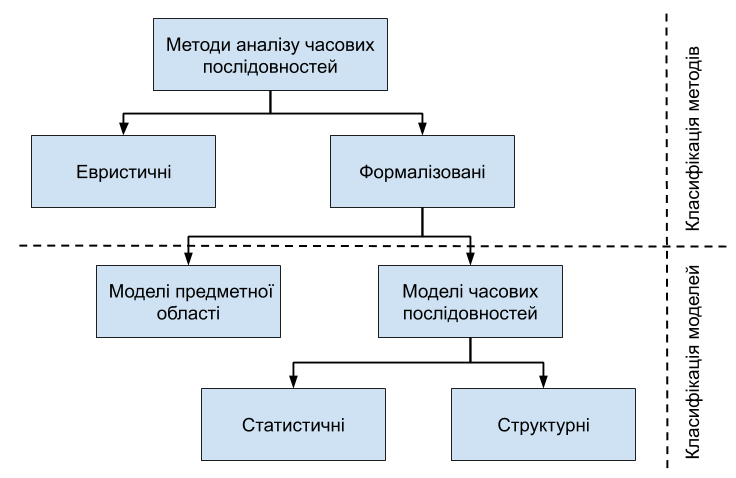
\includegraphics[scale=0.6]{method_model}
\caption{Класифікація методів та моделей аналізу часових послідовностей} 
\label{fig:method_model}
\end{center} \end{figure}

На рис.~\ref{fig:method_model} зображено класифікацію методів та моделей 
\cite{imp:Chuchueva2012}, де модель -- функціональне представлення, що з 
достатньою точністю описує досліджуваний процес, а метод являє собою 
послідовність дій які необхідно виконати для побудови моделі. Евристичні 
(інтуїтивні) методи аналізу базуються на судженнях і оцінках експертів, 
та використовуються в таких дисциплінах, як маркетинг, філософія, економіка 
і навряд підходять для виділення інформації з аналогового 
сигналу. Формалізовані методи дозволяють з заданою точністю побудувати 
математичну залежіть (модель), що пов'язує аналоговий сигнал та інформацію, 
що він несе. Доступні моделі розділяють на статистичні та структурні 
\cite{imp:Chuchueva2012}.

Моделі часових послідовностей базуються на методах, що шукають залежності
в середині самого нестаціонарного процесу і на цій основі виконують 
необхідний аналіз. Моделі часових послідовностей поділяються на статистичні
(регресія, EM-алгоритми, експоненційне стискання, еволюційні алгоритми, тощо)
та структурні (машинне навчання, ланцюги Маркова, класифікаційні дерева, 
узагальнене перетворення Хафа, каскади Хара, watershed, тощо). Статистичні 
моделі не придатні для застосування в розв'язанні задач виділення корисної 
інформації через їх алгоритмічну обчислювальну складність, натомість, 
константа складність деяких структурних алгоритмів робіть їх досить 
привабливими. Моделлю предметної області (радіофізики), у випадку виділення 
корисної інформації з сигналу, є послідовне застосування лінійного фільтра, 
низькошумного підсилювача, аналогово-цифрового перетворювача (АЦП) і модуля 
цифрової обробки FPGА, що переводить розв'язання в область структурної моделі
аналізу часової послідовності. В радіофізиці, такі методи застосовують як 
для задач локації \cite{imp:Dumin2017}, так і комунікації \cite{imp:Taok2009}.

Структурні моделі аналізу часових послідовностей, можна розділити за типом
інформації, що виділяється зі вхідних даних:

\begin{enumerate}

	\item Класифікація часової послідовності (Sequence classificaion). 
	Визначення приналежності сигналу, як цілого, до певного виду (класу) 
	з наперед відомими характеристиками. Активно застосовується в задачах 
	багатопроменевої і багатокористувацької надширокосмугової комунікації. 
	Прикладом найпростішого бінарного класифікатору є визначення наявності 
	сигналу за граничним значенням (threshold value), тобто на проміжках 
	спостереження, де значення досліджуваної функції більше за наперед 
	визначене значення, бінарний класифікатор вказує True, а в інших 
	випадках False.

	\item Маркування послідовності (Sequence labeling). Визначення 
	приналежності сигналу в кожен момент часу до певного виду з наперед 
	відомими характеристиками. Активно застосовується в задачах 
	багатопроменевої і багатокористувацької надширокосмугової комунікації.

	\item Пошук аномалей (Anomaly detection). Пошук проміжку часової 
	послідовності, який вибивається з загального вигляду даних та має 
	невизначену природу. Корисний для задач, де метод максимальної 
	правдоподібності застосувати неможливо через невизначеність 
	характеристик аномалії, що шукається, наприклад задачі автоматичного 
	визначення наявності випадкових завад невідомої природи.

	\item Передбачення послідовності (Sequence forcasting). Передбачення 
	значень часової послідовності засновуватись на минулих значеннях цієї 
	послідовності. В радіофізиці активно використовуються, як моделі з 
	учителем так і без.

	\item Генерація послідовності (Sequence generation). Генерація нової 
	часової послідовності на основі наявної з урахуванням зовнішніх факторів. 
	Генерація нової послідовності може проходити, як в порядку продовження 
	або доповнення існуючої, так і в порядку створення окремої послідовності.

	\item Фільтрування послідовності (Sequence filtering). Фільтрація 
	часової послідовності від завад або сторонніх сигналів, що вона 
	містить. Спосіб визначення завад та їх ліквідація залежить від 
	імплементації конкретної моделі. Найрозповсюдженіше сімейство моделей
	фільтрації часової послідовності в радіофізиці -- лінійна фільтрація, 
	наприклад: частотні фільтри, фільтр Калмана та узгоджений фільтр.

\end{enumerate}

З іншого боку, в здачах локації, інколи застосовують методи обробки 
зображень, формуючи карти інтенсивності з отриманого сигналу. Тобто,
задача аналізу часових послідовностей зводиться до задачі комп'ютерного зору. 
Через обчислювальну складність, такі методи застосовують лише в задачах де є 
необхідність накопичувати дані і в той самий час опрацьовувати готовий пакет 
даних вже готовий пакет даних. Таким чином, до структурних моделей 
аналізу часових послідовностей можна віднести, також, і деякі моделі 
аналізу зображень:

\begin{enumerate}

	\item Класифікація зображень (Image classificaion). Визначення 
	приналежності зображення, як цілого, до певного виду (класу) з наперед 
	відомими характеристиками.

	\item Детектування об'єктів (Object detetion). Визначення положень 
	обмежувальних прямокутників для об'єктів з наперед відомими 
	характеристиками, що містяться на зображені, яке досліджується.

	\item Сегментація об'єктів (Instance segmentation). Процес розділення 
	цифрового зображення на декілька сегментів довільної форми. Під сегментом 
	мається на увазі множина пікселів, які часто називають суперпікселями. 
	Така модель сегментації не розділяє об'єкти одного типу між собою.

	\item Семантична сегментація (Semantic segmentation). Процес розділення 
	цифрового зображення на декілька сегментів довільної форми, при тому, що
	форми об'єктів одного типу семантично розділені. Найрозповсюдженішим 
	підходом до семантичного розділення об'єктів є бінарні піксельні маски. 
	Типова модель для розв'язку таких задач -- штучна згорткова нейронна 
	мережа-автоенкодер UNet.

	\item Фільтрація зображення (Image filtering). Фільтрація зображення 
	від сторонніх шумів. Зручно застосовувати для отримання обробки 
	спектральних характеристик реальних сигналів 
	\textcolor{red}{[Коленов Дима]}.

\end{enumerate}

Для вибору класу моделі виділення інформації з сигналу, а також для 
дослідження даних і імплементації моделі прийнято застосовувати  
методологію аналізу даних CRISP-DM \cite{imp:CRISPDM2000}.


%%%%%%%%%%%%%%%%%%%%%%%%%%%%%%%%%%%%%%%%%%%%%%%%%%%%%%%%%%%%%%%%%%%%%%%%%%%%%%%
\section{Структурні моделі аналізу нестаціонарних процесів}

Фізичний процес -- зміна в часі деякої фізичної величини (інколи векторної). 
В теоретичній фізиці опис процесу найчастіше являє собою безперервну часову 
послідовність, що задано математичною функцією. На практиці -- дискретну часову 
послідовність, задану масивом значень змінної в часі величини. Структурною 
моделлю аналізу процесу називатимемо формалізовану модель, що виділяє з нього 
корисну інформацію засновуючись на закономірностях у зміні значень 
досліджуваної величини з плином часу.

Враховуючи шум в моделі інформаційного радіо-каналу \cite{imp:Shihovcev2011}, 
досліджуваний сигнал стає випадковим процесом, що ускладнює виділення 
корисної інформації для реальних задач. Джерелом шумів можуть бути як і 
зовнішні фактори (невідомі сторонні джерела електромагнітного поля) так і
саме обладнання прийму-передачі. Через це ускладнення базова інтуїтивна модель
виділення інформації, що базується на виявлені наявності сигналу за 
пороговим значенням напруженості струму стає малопридатною. Крім того,
додатковим фактором, що впливає на точність виділення інформації є розбіжності
протікання реального фізичного процесу передачі-поширення-прийму 
електромагнітного поля та моделі, що описує цей процес. Типовим способом 
розв'язання задач з вищезгаданими проблемами є застосування моделей з учителем
та калібрувальними параметрами.

% Прикладом такої нелінійної природи електромагнітного поля або ефектів ближньої 
% зони випромінювання призводить до спрощення моделі і викликає необхідність 
% В таких випадках застосовують методи з учителем, або калібрувальними 
% параметрами.

Основними критеріями вибору моделі стають обчислювальна складність її алгоритмів 
та точність самого методу. Для порівняння методів, а також для визначення їх 
абсолютної та відносної точності користаються широким класом метрик, але 
частіше доводиться визначати власні. Серед найчастіше вживаних метрик можна 
виділити середню абсолютну та квадратичну помилку \cite{imp:Willmott2005}, 
але через їх недоліки часто приходять до використання більш складних методів 
оцінки точності. Недоліки таких метрик часто допомагає вирішити логарифмізація 
значення середньої помилки і деякі регуляризації отриманої функції. 
Прикладом метрики в задачах класифікації можна навести F-метрики 
\cite{imp:Tharwat2018}, а для задач сегментації та індикації використовують 
Коэффициент Жаккара (Intercection Over Union або IoU) \cite{imp:Jaccard1901}.

% декілька методів одразу

Набір моделей, які можна застосувати до часових послідовностей, значно 
розширюється, якщо застосовувати методику ковзного вікна, тобто при аналізі 
безперервної часової послідовності розглядати одномоментно деякий проміжок 
дискретних значень, що рухається в часі. Наприклад, на вхід методу лінійної 
регресії \cite{imp:Xin2009} можна подати вектор, що складається з дискретних 
послівних значень взятих з деяким інтервалом з аналогового сигналу. Якщо 
інтервал і тривалість вікна будуть вибрані правильно, то модель лінійної
регресії можливо застосувати, щоб виявити наявність імпульсу. 

З приходом ери нейронних мереж \cite{imp:Rosenblatt1957}, їх застосування в
задачах дискримінантного аналізу витісняє інші методики. Так, для більш 
складних задач, таких як класифікація імпульсу, методика ковзного вікна 
дозволяє застосовувати повнозв'язані і згорткові нейронні мережі 
\cite{imp:Plakhtii2019}.

\begin{figure}[htbp] \begin{center}
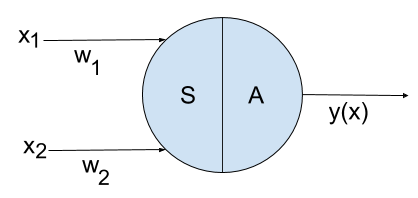
\includegraphics[scale=0.6]{perceptron}
\caption{Математична модель біологічного нейрону}
\label{fig:perceptron}
\end{center} \end{figure}

На рис.~\ref{fig:perceptron} зображено одну з математичних моделей (модель 
Розенблатта) біологічного нейрону. Вона виділяє дві функції нейрону: суматору 
і активаційну. Біологічній нейрон розглядають, як нелінійний пристрій з 
декількома вхідними інтерфейсами (дендритами) та єдиним вихідним (аксон).
Також сам нейрон характеризується своїм внутрішнім параметрам -- зміщення 
$ b $, який відповідає за порогове значення реагування нейрону. Суматора 
функція $ S $ в моделі нейрона описує механізм акумулювання довільної 
кількості ($ n $) вхідних сигналів, поєднаних в вектор $ \vect{x} $ 
розмірністю $ n + 1 $, де останній елемент вектору завжди $ 1 $:

\begin{equation}
\func{S}{\vect{x}} = \vect{w}^\intercal \vect{x},
\end{equation}
%
де $ \vect{w}^\intercal = \left( w_1, w_2, ..., w_n, b \right) $, а
$ \vect{x} = \left( x_1, x_2, ..., x_n, 1 \right)^\intercal $.
Активаційна функція $ \func{A}{\func{S}{\vect{x}}} $ описує механізм 
реагування на акумульовані вхідні сигнали. Для класичного перцептрону 
активаційною є функція Хевісайда. Також часто застосовують сигмоїдальні 
активаційні функції та функції ReLu \cite{imp:Kussul2004}.

Разом з розповсюдженням аналогової радіоелектроніки почали заявлятись 
структурні моделі пристосовані саме для аналізу аналогових сигналів 
та часових послідовностей \cite{imp:Markov1906}. Проривом стала можливість
зберігати минулі значення послідовності у якості стану системи 
(ланцюга Маркова) і на основі цього стану проводити аналіз поточного 
значення випадкового процесу. Такий підхід дозволив скоротити кількість 
параметрів моделі у порівнянні з лінійною регресією. У порівнянні з 
багатошаровим перцептроном модель, ланцюгів Маркова показувала низьку 
запам'ятовувальну здатність, а тому в складних задачах розрізнення великої 
кількості класів показувала гірші результати.

Лише поява рекурентних нейронних мереж у 1988 році \cite{imp:Rumelhart1988} 
дозволила застосовувати на практиці моделі, що зберігають інформацію про 
випадковий процес в якості свого внутрішнього стану і не потребують 
застосування методу ковзного вікна. Цей метод та подальші його модифікації
стали перспективним напрямком розвитку структурних моделей аналізу процесів. 


%%%%%%%%%%%%%%%%%%%%%%%%%%%%%%%%%%%%%%%%%%%%%%%%%%%%%%%%%%%%%%%%%%%%%%%%%%%%%%%
\section{Рекурентні нейронні мережі тривалої короткочасної пам'яті для 
обробки нестаціонарних сигналів}

Рекурентна нейронна мережа може бути представлена, як ланцюг, що складається
з ланок (штучних нейронів), які відрізняються одна від одної лише своїм 
внутрішнім станом (рис.~\ref{fig:rnn_unrolled}). Принцип роботи цієї моделі 
засновано на типовому для радіофізики фізичному принципі зворотнього зв'язку:
вихідне значення мережі в поточний момент часу вливає на її вихідне значення 
в майбутньому.

\begin{figure}[htbp] \begin{center}
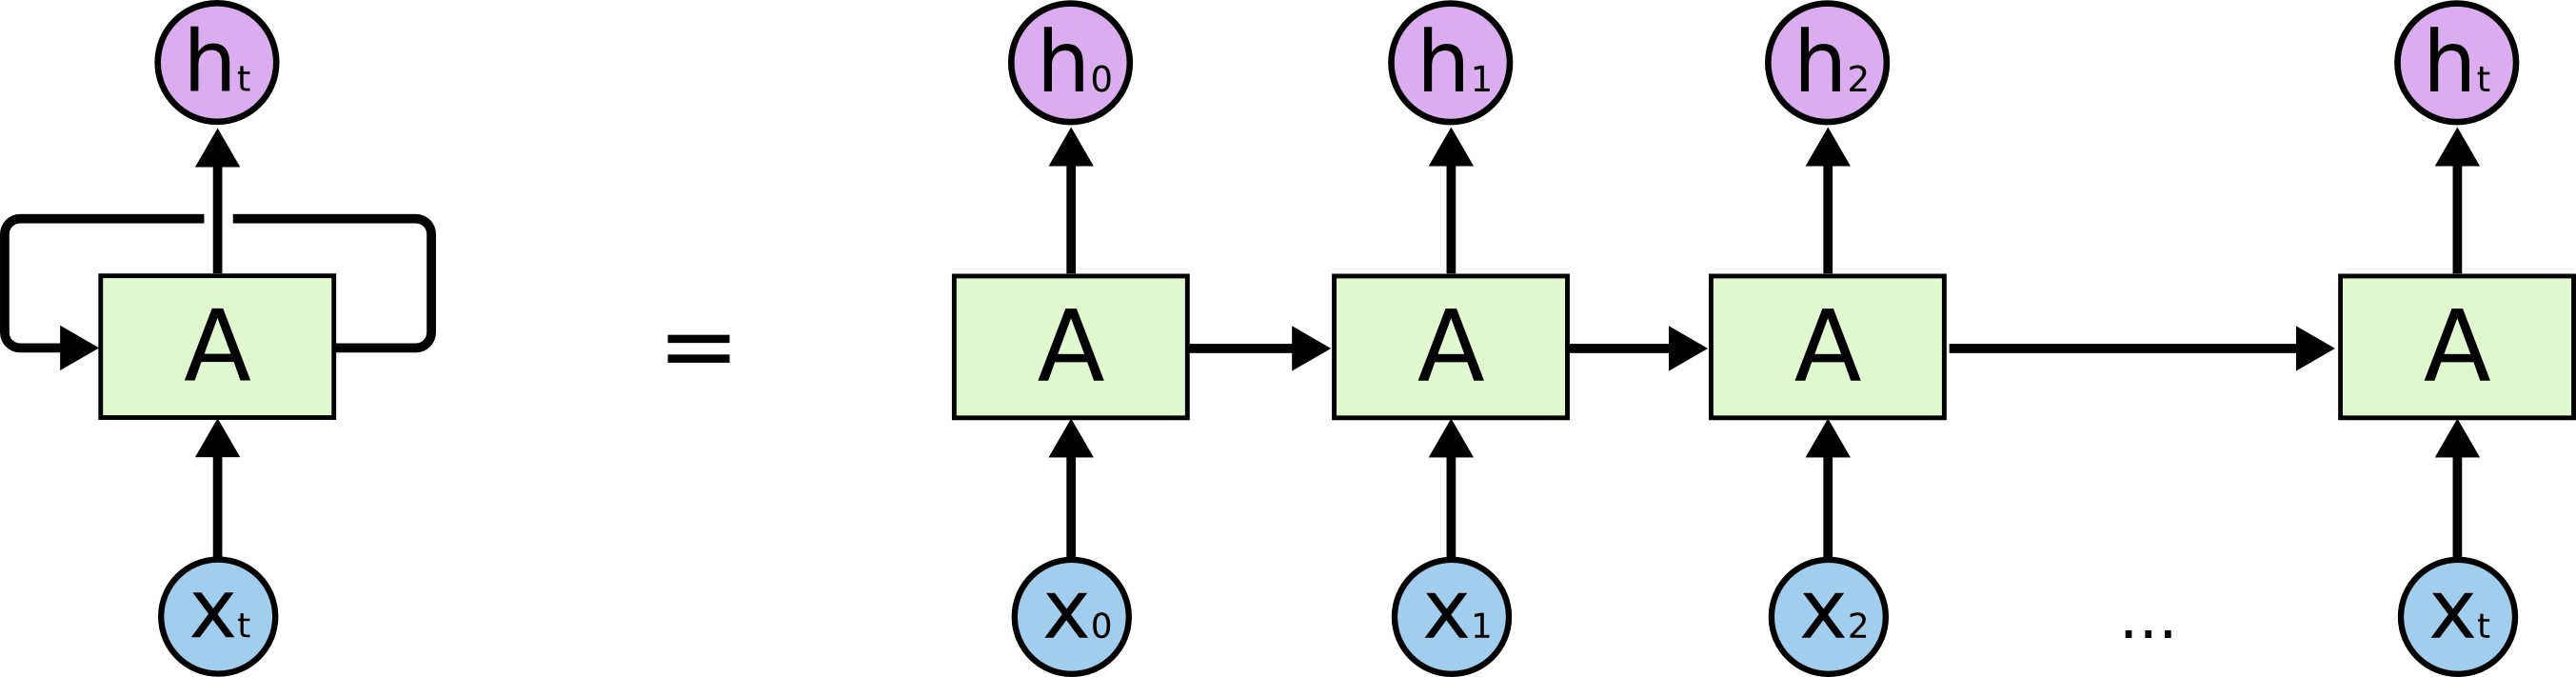
\includegraphics[scale=0.4]{rnn_unrolled}
\caption{Проходження сигналу крізь рекурентну нейронну мережу}
\label{fig:rnn_unrolled}
\end{center} \end{figure}

На рис.~\ref{fig:rnn_unrolled} літерою А позначено ланку ланцюга, $ x_i $ --
дискретне значення вхідної часової послідовності (вхід), а $ h_t $ -- якісна 
або кількісна характеристика виділена нейронною мережею з сигналу (вихід). 
На відміну від класичного перцептрону Розенблатта, ланки рекурентного ланцюга 
мають додатковий вихід, що передає свій внутрішній стан на наступну ланку.

Входом для такої математичної моделі є дискретизована часова послідовність 
довільної тривалості. Виходом також є часова послідовність, але не завжди з 
таким же періодом дискретизації. 

Випадок, коли частота дискретизації входу та виходу співпадає, тобто кожному 
елементу вхідної послідовності $ x_i $ підставляється окремий елемент 
вихідної $ h_i $ є найчастіше вживаним в радіофізиці. Тут кожен дискретний 
вихід моделі $ h_i $ базується на проміжку даних 
$ \left[ x_{i-j} , x_i \right] $, де $ j $ -- довільна 
кількість врахованих елементів входу, яка обмежена максимальною 
запам'ятовувальною знатністю моделі. Зазвичай, максимальна 
запам'ятовувальна знатність є гіперпараметром тренувального алгоритму 
рекурентрої мережі. Моделі такого типу відомі в закордонній літературі, як 
many-to-many.

Також зустрічаються моделі для яких частота дискретизації входу та виходу 
не співпадає. В моделях де одному вхідному дискретному значенню 
співставляєтья деякий проміжок вихідної послідовності називають one-to-many.
Прикладом one-to-many задачі є підвищення якості звуку. Задачі, в яких 
навпаки, деякому проміжку вхідних значень $ \left[ x_{i-N} , x_i \right] $, 
де $ N $ -- стала константа, співставляється одне вихідне значення $ h_i $
називають many-to-one. На відміну від many-to-many задач, тут 
дискретне вихідне значення базується на проміжку вхідних даних сталої 
тривалості, що накладає деякі обмеження на застосування моделі. Такий 
підхід еквівалентний застосуванню методики ковзного вікна.

Підхід із застосуванням медики ковзного вікна має суттєвий недолік: 
тривалість вікна залишається сталою, коли тривалість сигналу залежить від 
багатьох факторів, а отже вибирати тривалість вікна треба з огляду на 
максимально можливу тривалість імпульсу. Це призводить до того, що для 
більш коротких імпульсів модель може втратити точність. В задачах локації, 
де корисна інформація знаходиться в післяімпульсних коливаннях, тривалість 
яких взагалі не обмежена, застосування методики ковзного вікна принципово 
неможливе без обмеження на глибину зондування.

Сьогодні, прижились дві реалізації ланок рекурентних мереж, які застосовують,
як для many-to-one так і для many-to-many -- це LSTM та GRU, які дуже схожі 
за своїми можливостями. Класичні RNN без механізму забування вважаються менш 
ефективними через низьку максимальну запам'ятовувальну знатність.

\begin{figure}[htbp] \begin{center}
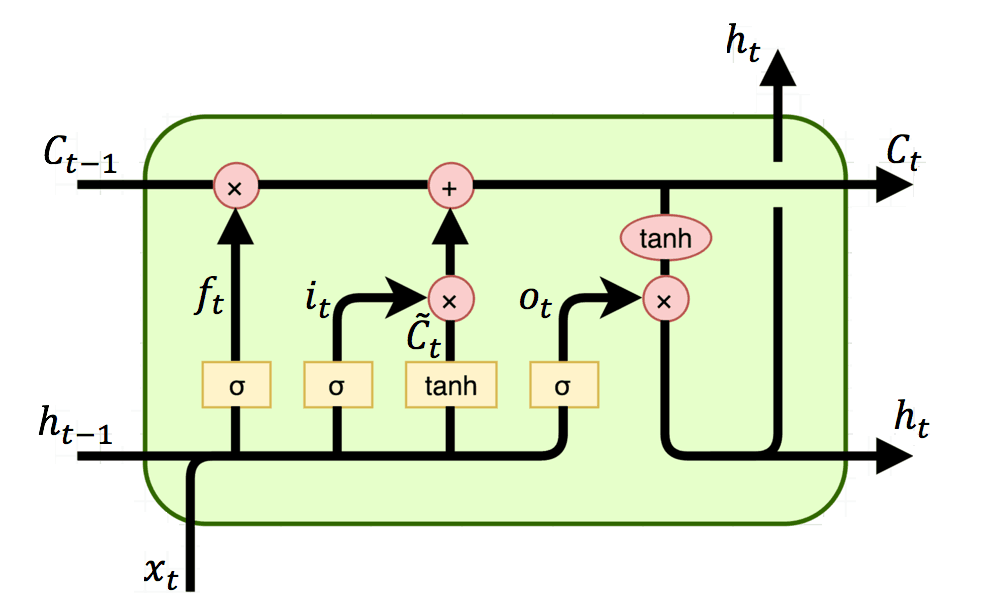
\includegraphics[scale=0.5]{lstm_inside}
\caption{Внутрішня структура ланки ланцюга LSTM}
\label{fig:lstm_inside}
\end{center} \end{figure}

На рис.~\ref{fig:lstm_inside} з \cite{imp:Varsamopoulos2018} зображено 
внутрішню будову ланки рекурентної мережі довготривалої та короткотривалої 
пам'яті. Символом множення на рисунку позначена операція множення чисел, а 
плюсом -- додавання. Також, жовтими прямокутниками позначено функції, що діють 
на число: $ \tanh $ -- гіперболічний тангенс та $ \sigma $ -- сигмоїда.

Передача внутрішнього стану $ C_t $ на наступну ланку здійснюється по 
верхній горизонтальній стрілці, де цей внутрішній стан змінюється на основі
поточного значення вхідної часової послідовності $ x_t $ та передбачення 
моделі на минулій ланці $ h_{t-1} $.

Першим етапом обробки часової послідовності є так званий поріг забування
(або forget gate). При проходженні крізь нього ми визначаємо яку 
кількість інформації про часову послідовність слід забути:

\begin{equation}
f_t = \func{\sigma}{\dotprod{W_f}{\crossprod{h_{t-1}}{x_t}} + b_f},
\end{equation}
%
де $ W_f $ і $ b_f $ -- матричні тренувальні параметри.

Наступний етап визначає на скільки потенційно важливим може стати поточне 
значення нейронної мережі та чи треба зберігати його у внутрішньому стані. 
Цей етап називають прохідний поріг (або input gate):

\begin{equation}
i_t = \func{\sigma}{\dotprod{W_i}{\crossprod{h_{t-1}}{x_t}} + b_i},
\end{equation}

\begin{equation}
\tilde{C_t} = \func{\tanh}{\dotprod{W_C}{\crossprod{h_{t-1}}{x_t}} + b_C},
\end{equation}
%
де $ W_C, b_C $ -- матричні тренувальні параметри.

Користуючись отриманими значеннями прохідного порогу і порогу забування
можна змінити внутрішній стан моделі:

\begin{equation}
C_t = f_t C_{t-1} + i_t \tilde{C_t}.
\end{equation}

Отримавши новий внутрішній стан моделі $ C_t $ можна отримати поточне вихідне 
значення (передбачення) $ h_t $ користуючись поточним вхідним значенням 
$ x_t $ послідовності, як порогом забування:

\begin{equation}
o_t = \func{\sigma}{\dotprod{W_o}{\crossprod{h_{t-1}}{x_t}} + b_o},
\end{equation}

\begin{equation}
h_t = o_t \func{\tanh}{C_t},
\end{equation}
%
де $ W_o, b_o $ -- матричні тренувальні параметри.

Алгоритмом зворотнього поширення помилки знаходять тренувальні 
параметри $ W_f, b_f, W_C, b_C, W_o, b_o $. На відміну від повнозв'язних ШНМ, 
алгоритм зворотнього поширення помилки повинен враховувати не лише пари даних 
входу та виходу моделі, а ще проміжний результат у вигляді зміни внутрішнього 
стану нейронної мережі $ \partder{C_t}{x_t} $.
